\subsection{Tecnologie}
\begin{itemize}
    \item \textbf{Python} \textit{(Faker o simili)}\textbf{:} Per la simulazione delle informazioni provenienti dai sensori.
    \item \textbf{Apache Kafka:} Broker per disaccoppiare lo stream di informazioni provenienti dai simulatori dei sensori.
    \item \textbf{ClickHouse:} database \textit{OLAP} per mantenere i numerosi dati provenienti dai sensori.
    \item \textbf{Grafana:} piattaforma di Data Visualization per permettere il monitoraggio della città e la visualizzazione delle informazioni raccolte dai sensori.
\end{itemize}

\begin{figure}[H]
    \centering
    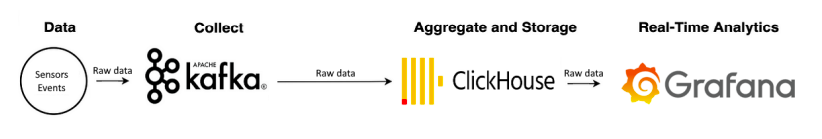
\includegraphics[width=0.9\textwidth]{../Images/stackTecnologico.PNG}
    \caption{Stack tecnologico}
    \label{fig:stackTecnologico}
\end{figure}
